% Scheme of the three-layer model of cognitive tasks involved while driving.
% The figure illustrates the Hierarchical Control Model proposed by Michon.
%
\documentclass{standalone}
\usepackage{tikz}

\begin{document}
	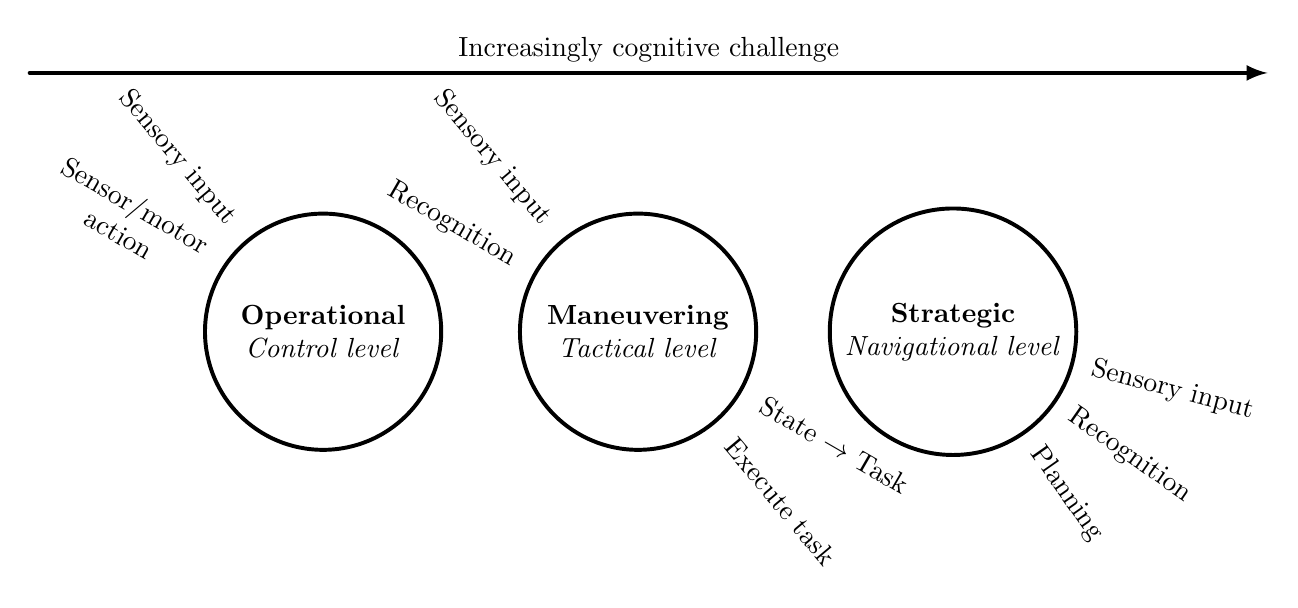
\begin{tikzpicture}[
	line cap=round,
	line join=round,
	>=latex,
	every node/.style={align=center},
	challenge/.style={
		shape=circle,
		minimum size=3cm,
		line width=0.05cm,
		draw,
		text centered
	}
	]
	\begin{scope}[local bounding box=lifecycle]
	\begin{scope}[shift=(0:0)]
	\node [challenge] (data) {
		\textbf{Operational}
		\\
		\textit{Control level}
	};
	\foreach \characteristic [count=\i, evaluate={\a=\i*20+110;}] in {Sensory input, Sensor/motor\\ action}{
		\node at (\a:1.7cm) [rotate=\a+180, anchor=east] {\characteristic};
	}
	\end{scope}
	\begin{scope}[shift=(0cm:4cm)]
	\node [challenge] (process) {
		\textbf{Maneuvering}
		\\
		\textit{Tactical level}
	};
	\foreach \characteristic [count=\i, evaluate={\a=\i*20+110;}] in
	{Sensory input, Recognition}{
		\node at (\a:1.7cm) [rotate=\a+180, anchor=east] {\characteristic};
	}
	\foreach \characteristic [count=\i, evaluate={\a=-\i*20-10;}] in
	{State $\rightarrow$ Task, Execute task}{
		\node at (\a:1.7cm) [rotate=\a, anchor=west] {\characteristic};
	}
	\end{scope}
	\begin{scope}[shift=(0cm:8cm)]
	\node [challenge] (management) {
		\textbf{Strategic}
		\\
		\textit{Navigational level}
	};
	\foreach \characteristic [count=\i, evaluate={\a=70-\i*20-65;}] in
	{Sensory input, Recognition, Planning}{
		\node at (\a:1.7cm) [rotate=\a, anchor=west] {\characteristic};
	}
	\end{scope}
	\end{scope}
	\draw [ultra thick, ->] (lifecycle.north west) -- (lifecycle.north east)
	node [midway, above] {Increasingly cognitive challenge};
	
	\end{tikzpicture}
\end{document}

